\begin{center}
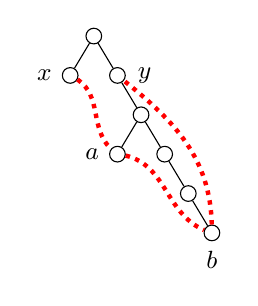
\begin{tikzpicture}[scale=.5,level distance=10mm, state/.style={circle, draw, minimum size=1mm}]]
  \tikzstyle{every node}=[font=\small, draw=black,circle,inner sep=2pt, minimum size=1mm]
  \tikzstyle{level 1}=[sibling distance=12mm, set style={{every node}+=[draw=black]}]
  \tikzstyle{level 2}=[sibling distance=12mm, set style={{every node}+=[draw=black]}]
  \tikzstyle{level 3}=[sibling distance=12mm,  set style={{every node}+=[draw=black]}]

    \node {}
     child {
        node[label=left:{$x$}] (x) {}}
            child{ node[label=right:{$y$}] (y) {}
            child[fill=none] {edge from parent[draw=none]}
            child{node {}
            child{node[label=left:{$a$}] (a) {}}
            child{node {}
            child[fill=none] {edge from parent[draw=none]}
            child{node {}
            child[fill=none] {edge from parent[draw=none]}
            child{node[label=below:{$b$}] (b) {}
            }
            }}
            }
            };
    
    \draw[-,dotted,ultra thick,relative,red] (x) to[out=30,in=200] (a);

    \draw[-,dotted,ultra thick,relative,red] (a) to[out=30,in=200] (b);
    
    \draw[-,dotted,ultra thick,relative,red] (b) to[out=-30,in=200] (y);
       
\end{tikzpicture}
\end{center}